\documentclass{beamer}
% \usepackage{moreverb} 
\usepackage{listings}
\usepackage{mflogo}

\mode<presentation> {
  \usetheme{Warsaw}
  \setbeamercovered{opaque}
}

\usebackgroundtemplate{
\includegraphics[width=\paperwidth]{format/libresoft-bg.png}}
\usepackage[spanish]{babel}
\usepackage[utf8]{inputenc}
\usepackage{graphics}
\usepackage{amssymb} % Simbolos matematicos

%% Metadatos del PDF.
\hypersetup{  
  pdftitle={Xen: Curso práctico},
  pdfauthor={Jose Castro},
  pdfcreator={GSyC/Libresoft},
  pdfproducer=PDFLaTeX,
  pdfsubject={Master on Free Software},
}
%%

\defbeamertemplate*{footline}{shadow theme}
{%
  \leavevmode%
  \hbox{\begin{beamercolorbox}[wd=.5\paperwidth,ht=2.5ex,dp=1.125ex,leftskip=.1cm plus1fil,rightskip=.2cm]{author in head/foot}%

\includegraphics[scale=0.40]{format/cc-by-80x15.png} \hspace{0.05cm}
	Miguel Vidal / Jose Castro
  \end{beamercolorbox}%
  \begin{beamercolorbox}[wd=.5\paperwidth,ht=2.5ex,dp=1.125ex,leftskip=.3cm,rightskip=.3cm plus1fil]{title in head/foot}%
    \usebeamerfont{title in head/foot}\insertshorttitle%
    \hspace{2cm} \usebeamerfont{author in head/foot}\insertframenumber\,/\,\inserttotalframenumber\hfill
  \end{beamercolorbox}}%
  \vskip0pt%
}


\begin{document}

\title{Xen: Curso práctico}
\subtitle{System Integration}
% \institute{\texttt{http://gsyc.urjc.es/\~{}mvidal} \\ Twitter: \texttt{@mvidallopez}}
\author{Miguel Vidal, Jose Castro} 
\date{\footnotesize{Master on Free Software \\ April 20th, 2012}}
\author{Miguel Vidal \hspace{1cm} Jose Castro \\
\hspace{0.5mm} {\tiny Twitter: @mvidallopez \hspace{1.1cm}Twitter: @jfcastroluis}
}


\frame{
\maketitle
\begin{center}

\includegraphics[width=6cm]{format/gsyc-urjc}
\end{center}
}

%% License slide
\begin{frame}
  \vspace{2cm}
  \begin{flushright}
    {\small \copyright{} 2010-2012 Miguel Vidal, Jose Castro} \\
%    \vspace{0.25cm}
    \medskip
    {\scriptsize This work is licensed under \\ a Creative Commons Attribution 3.0 License}
%    \vspace{0.10cm}
  \end{flushright}
  \begin{flushright}
    \href{http://creativecommons.org/licenses/by/3.0/es}{
\includegraphics[width=2cm]{format/cc-by.png}} \\
    {\tiny \url{http://creativecommons.org/licenses/by/3.0}}
  \end{flushright}
\end{frame}%%

\usebackgroundtemplate{}

\AtBeginSection[]
{
\begin{frame}<beamer>
\begin{center}
{\huge \insertsection}
\end{center}
\end{frame}
}

\AtBeginSection[]
{
  \begin{frame}<beamer>{Índice}
    \tableofcontents[currentsection]
  \end{frame}
}


\AtBeginSubsection[]
{
  \begin{frame}<beamer>{Índice}
    \tableofcontents[currentsection,currentsubsection]
  \end{frame}
}

%%

%%%%%%%%%%%%%%%%%%%%%%%%%%%%%%%%%%%%%%%%%%%%%%%%%%%%%%%%%%%%%%%%%%%%%%%

\section{Fundamentos de Xen}


\begin{frame}
\frametitle{Xen: Características (1)}

\begin{itemize}
\item Xen utiliza \alert{paravirtualización}.
\item El sistema operativo huésped tiene que estar modificado para usar el hipervisor.
\item También admite virtualización completa (con Intel VT o AMD-V): 
	\begin{itemize}
	\item huéspedes sin modificar 
	\item permite que sistemas operativos privativos (como Windows) puedan ser virtualizados.
	\end{itemize}
\end{itemize}

\end{frame}

%%%%%%%%%%%%%%%%%%%%%%%%%%%%%%%%%%%%%%%%%%%%%%%%%%%%%%%%%%%%%%%%%%%%%%%

\begin{frame}
\frametitle{Xen: Características (2)}

\begin{itemize}
\item Es capaz de hacer \alert{migración} de máquinas virtuales.
\item Xen (HV) se ejecuta en el anillo de protección 0 mientras que los dominios se ejecutan en el anillo 1 o anillo 3.

\begin{figure}
  \centering
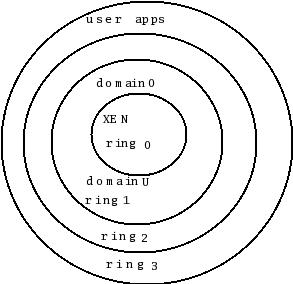
\includegraphics[scale=0.40,clip=false]{figs/rings-xen.png}
  \caption{\footnotesize{Anillos: dominios de protección jerárquica (x86)}}
\end{figure}

\end{itemize}

\end{frame}


%%%%%%%%%%%%%%%%%%%%%%%%%%%%%%%%%%%%%%%%%%%%%%%%%%%%%%%%%%%%%%%%%%%%%%%

\begin{frame}
\frametitle{Xen: Prestaciones (1)}
\begin{itemize}

\item \alert{Independencia} entre los sistemas virtualizados. Se puede reiniciar y crear independientemente.
\item \alert{Uso mejorado del hardware}: balanceo de recursos. Una máquina virtual puede hacer uso de los recursos que no utilizan las otras máquinas virtuales.
\item \alert{Backup sencillo}. Sólo con copiar la máquina virtual se puede levantar en un nuevo servidor. Xen también permite la migración en caliente, siendo muy flexible y minimizando el tiempo de recuperación en caso de fallo.
\end{itemize}

\end{frame}

%%%%%%%%%%%%%%%%%%%%%%%%%%%%%%%%%%%%%%%%%%%%%%%%%%%%%%%%%%%%%%%%%%%%%%%

\begin{frame}
\frametitle{Xen: Prestaciones (2)}
\begin{itemize}

\item Se pueden \alert{modificar parámetros} como la RAM, el número de CPUs y el espacio en disco para cada necesidad específica de cada máquina virtual.
\item \alert{Entornos de prueba} y desarrollo: múltiples máquinas virtuales en un único servidor físico para probar y desarrollar.
\end{itemize}

\end{frame}


%%%%%%%%%%%%%%%%%%%%%%%%%%%%%%%%%%%%%%%%%%%%%%%%%%%%%%%%%%%%%%%%%%%%%%%

\begin{frame}
\frametitle{Xen: Cómo funciona}
\begin{center}
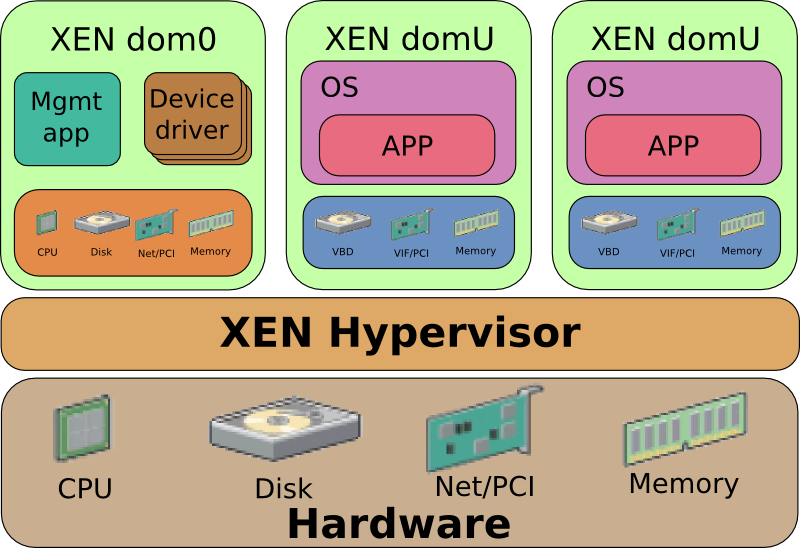
\includegraphics[width=9cm]{figs/XEN-schema.png}
\end{center}
\end{frame}

%%%%%%%%%%%%%%%%%%%%%%%%%%%%%%%%%%%%%%%%%%%%%%%%%%%%%%%%%%%%%%%%%%%%%%%

\begin{frame}
\frametitle{¿Xen integrado en Linux?}

\vspace{-0.25cm}
\begin{center}
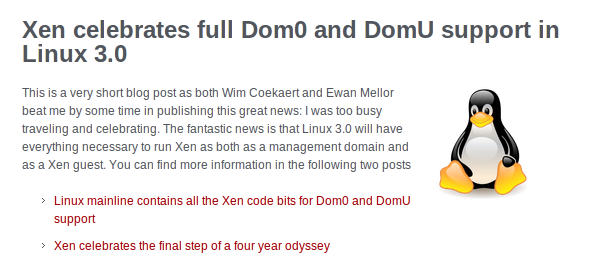
\includegraphics[width=5.5cm]{figs/xen-kernel-support.png} \\
\end{center}

\begin{flushright}
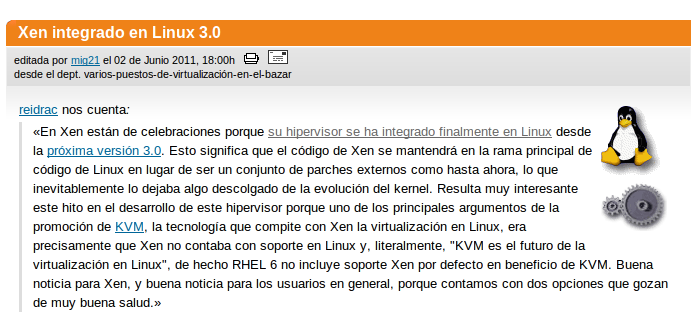
\includegraphics[width=5.5cm]{figs/xen-kernel-support3.png} \\
\end{flushright}

\begin{center}
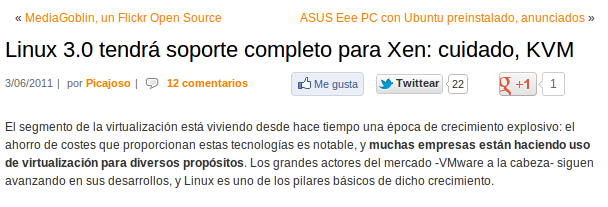
\includegraphics[width=5cm]{figs/xen-kernel-support2.png} 
\end{center}

\end{frame}


%%%%%%%%%%%%%%%%%%%%%%%%%%%%%%%%%%%%%%%%%%%%%%%%%%%%%%%%%%%%%%%%%%%%%%%

\begin{frame}
\frametitle{Xen: Linux 3.0}
\begin{itemize}

\item En Linux 3.0 los \alert{drivers paravirtualizados de Xen} se integran en el kernel oficialmente.
\item Ahora pueden usarse Dom-0 (host) y DomU sin modificar/hackear el kernel.
\item El hipervisor Xen sigue siendo un proyecto desarrollado aparte de Linux.
\item KVM sigue siendo el único hipervisor integrado en el kernel Linux.
\end{itemize}

\end{frame}

%%%%%%%%%%%%%%%%%%%%%%%%%%%%%%%%%%%%%%%%%%%%%%%%%%%%%%%%%%%%%%%%%%%%%%%

\begin{frame}
\frametitle{Xen en kernel Linux 2.x}
\begin{center}
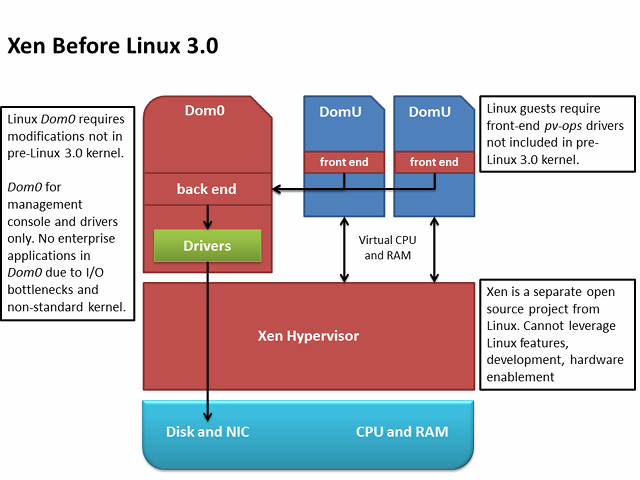
\includegraphics[width=9cm]{figs/xen-old-kernels.png}
\end{center}
\end{frame}

%%%%%%%%%%%%%%%%%%%%%%%%%%%%%%%%%%%%%%%%%%%%%%%%%%%%%%%%%%%%%%%%%%%%%%%

\begin{frame}
\frametitle{Xen en kernel Linux 3.x}
\begin{center}
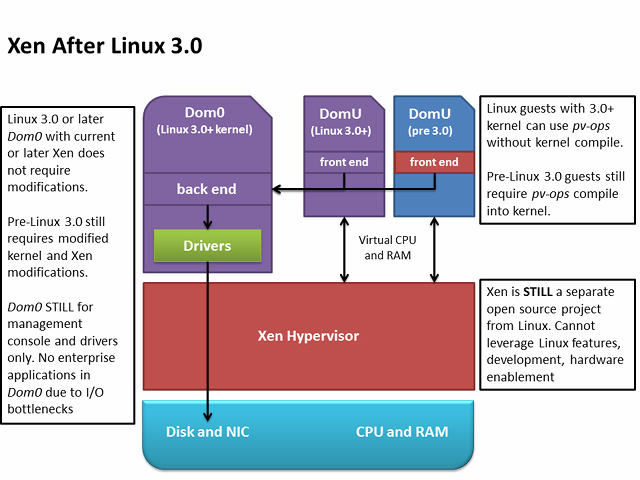
\includegraphics[width=9cm]{figs/xen-new-kernel.png}
\end{center}
\end{frame}



%%%%%%%%%%%%%%%%%%%%%%%%%%%%%%%%%%%%%%%%%%%%%%%%%%%%%%%%%%%%%%%%%%%%%%%
\section{Instalación}
%%%%%%%%%%%%%%%%%%%%%%%%%%%%%%%%%%%%%%%%%%%%%%%%%%%%%%%%%%%%%%%%%%%%%%%

\begin{frame}
  \frametitle{Instalación}
  \begin{block}{Instalación del sistema}
    \texttt{\# apt-get install xen-hypervisor-4.1-amd64 xen-utils-4.1 [bridge-utils]}
    \begin{itemize}
      \item xen-hypervisor-4.1-amd64 --- hipervisor
      \item xen-utils-4.1 --- utilidades para la gestión
      \item bridge-utils --- utilidades de red para \textit{bridges}
    \end{itemize}
    \bigskip
  \end{block}
  Debemos reiniciar con el kernel de Xen
\end{frame}
%%%%%%%%%%%%%%%%%%%%%%%%%%%%%%%%%%%%%%%%%%%%%%%%%%%%%%%%%%%%%%%%%%%%%%%

\begin{frame}[fragile]
  \frametitle{Comprobación}
  \begin{block}{virsh}
    \texttt{\# virsh -c xen:/// list} \\
    \small{\begin{verbatim}
Id Name                  State
----------------------------------
 0 Domain-0             running
    \end{verbatim}}
  \end{block}
  \bigskip
  \begin{block}{xm}
    \texttt{\# xm list} \\
    \tiny{\begin{verbatim}
Name                              ID   Mem VCPUs      State   Time(s)
Domain-0                           0  1887     2     r-----    599.0
    \end{verbatim}}
  \end{block}
\end{frame}
%%%%%%%%%%%%%%%%%%%%%%%%%%%%%%%%%%%%%%%%%%%%%%%%%%%%%%%%%%%%%%%%%%%%%%%

\begin{frame}[fragile]
  \frametitle{Herramientas}
  \begin{block}{Xen tools}
    \texttt{\# apt-get install xen-tools}
  \end{block}
  \begin{block}{/etc/xen-tools/xen-tools.cfg}
    \tiny{\begin{verbatim}
dir = /home/xen

install-method = debootstrap

size   = 5Gb       # Disk image size.
memory = 512Mb     # Memory size
swap   = 512Mb     # Swap size
fs     = ext3      # use the EXT3 filesystem for the disk image.
dist   = squeeze   # Default distribution to install.
image  = full      # Specify sparse vs. full disk images.

passwd = 1

mirror = http://ftp.es.debian.org/debian/
    \end{verbatim}}
  \end{block}
\end{frame}
%%%%%%%%%%%%%%%%%%%%%%%%%%%%%%%%%%%%%%%%%%%%%%%%%%%%%%%%%%%%%%%%%%%%%%%

%%%%%%%%%%%%%%%%%%%%%%%%%%%%%%%%%%%%%%%%%%%%%%%%%%%%%%%%%%%%%%%%%%%%%%%
\section{Configuración}
%%%%%%%%%%%%%%%%%%%%%%%%%%%%%%%%%%%%%%%%%%%%%%%%%%%%%%%%%%%%%%%%%%%%%%%

\begin{frame}[fragile]
  \frametitle{Modo NAT}
  \begin{block}{/etc/xen/xend-config.spx}
    \texttt{(network-script network-nat)} \\
    \texttt{(vif-script vif-nat)} \\
    \medskip
    \texttt{(dom0-min-mem 196) } \\
    \medskip
    \texttt{(dom0-cpus 0)} \\
    \medskip
    \texttt{(vnpasswd '')}
  \end{block}
  \bigskip
  \begin{center}
    \texttt{\# service xend restart}
  \end{center}
\end{frame}
%%%%%%%%%%%%%%%%%%%%%%%%%%%%%%%%%%%%%%%%%%%%%%%%%%%%%%%%%%%%%%%%%%%%%%%

%%%%%%%%%%%%%%%%%%%%%%%%%%%%%%%%%%%%%%%%%%%%%%%%%%%%%%%%%%%%%%%%%%%%%%%
\section{Gestión de Máquinas Virtuales}
%%%%%%%%%%%%%%%%%%%%%%%%%%%%%%%%%%%%%%%%%%%%%%%%%%%%%%%%%%%%%%%%%%%%%%%

\begin{frame}
  \frametitle{Creación}
  \begin{block}{Creación VM}
    \# xen-create-image $--$hostname=webserver $--$dhcp 
  \end{block}
  \begin{itemize}
    \item Configuración: \texttt{/etc/xen/webserver.cfg}
    \item Imagen: \texttt{/home/xen/domains/webserver/}
  \end{itemize}
\end{frame}
%%%%%%%%%%%%%%%%%%%%%%%%%%%%%%%%%%%%%%%%%%%%%%%%%%%%%%%%%%%%%%%%%%%%%%%

\begin{frame}[fragile]
  \frametitle{Arranque}
  \begin{block}{Arranque VM}
    \texttt{\# xm create webserver.cfg [-c]} \\
  \end{block}
  \bigskip
  \begin{block}{Arranque automático}
    \texttt{\# cd /etc/xen/auto} \\
    \texttt{\# ln -s ../webserver.cfg webserver.cfg} \\
  \end{block}
\end{frame}
%%%%%%%%%%%%%%%%%%%%%%%%%%%%%%%%%%%%%%%%%%%%%%%%%%%%%%%%%%%%%%%%%%%%%%%

\begin{frame}
  \frametitle{Consola}
  \begin{block}{Consola}
    \texttt{\# xm console webserver}
  \end{block}
  \bigskip
  Para salir \texttt{Ctrl + AltGr + $]$}
\end{frame}
%%%%%%%%%%%%%%%%%%%%%%%%%%%%%%%%%%%%%%%%%%%%%%%%%%%%%%%%%%%%%%%%%%%%%%%

\begin{frame}
  \frametitle{Parada}
  \begin{block}{Parada VM}
    \texttt{\# xm shutdown webserver}
  \end{block}
  \bigskip
  \begin{block}{Botonazo VM}
    \texttt{\# xm destroy webserver}
  \end{block}
\end{frame}
%%%%%%%%%%%%%%%%%%%%%%%%%%%%%%%%%%%%%%%%%%%%%%%%%%%%%%%%%%%%%%%%%%%%%%%

\begin{frame}
  \frametitle{Borrado}
  \begin{block}{Borrado VM}
    \texttt{\# xm shutdown webserver} \\
  \end{block}
  \bigskip
  \begin{block}{Borrado ficheros}
    \texttt{\# rm -r /home/xen/domains/webserver/} \\
    \texttt{\# rm /etc/xen/auto/webserver.cfg} \\
    \texttt{\# rm /etc/xen/webserver.cfg} \\
  \end{block}
\end{frame}
%%%%%%%%%%%%%%%%%%%%%%%%%%%%%%%%%%%%%%%%%%%%%%%%%%%%%%%%%%%%%%%%%%%%%%%

\begin{frame}
  \frametitle{Comandos básicos}
  \begin{itemize}
    \item \textbf{xm help}: muestra la ayuda del comando
    \item \textbf{xm list}: listado de dominios activos
    \item \textbf{xm info}: muestra información del dom0
    \item \textbf{xm top}: muestra información de los dominios
    \item \textbf{xm pause}: parar temporalmente un dominio
    \item \textbf{xm unpause}: vuelve a la actividad un dominio suspendido
    \item \textbf{xm save}: guarda un dominio ejecutando en un fichero
    \item \textbf{xm restore}: crea un dominio desde un fichero
    \item \textbf{xm migrate}: migra un dominio a otro host
  \end{itemize}
\end{frame}
%%%%%%%%%%%%%%%%%%%%%%%%%%%%%%%%%%%%%%%%%%%%%%%%%%%%%%%%%%%%%%%%%%%%%%%

\begin{frame}
  \frametitle{GUI}
  \begin{block}{virt-manager}
    \texttt{\# apt-get install virt-manager}
  \end{block}
  \bigskip
  \begin{itemize}
    \item Permite gestionar los dominios virtuales
%    \item Permite conexiones locales y remotas
    \item Es una interfaz gráfica realmente completa
  \end{itemize}
\end{frame}
%%%%%%%%%%%%%%%%%%%%%%%%%%%%%%%%%%%%%%%%%%%%%%%%%%%%%%%%%%%%%%%%%%%%%%%

%%%%%%%%%%%%%%%%%%%%%%%%%%%%%%%%%%%%%%%%%%%%%%%%%%%%%%%%%%%%%%%%%%%%%%%
\section{Almacenamiento externo}
%%%%%%%%%%%%%%%%%%%%%%%%%%%%%%%%%%%%%%%%%%%%%%%%%%%%%%%%%%%%%%%%%%%%%%%

\begin{frame}
  \frametitle{Creación fichero}
  \begin{block}{Creación fichero almacenamiento}
    \small{\texttt{\# dd if=/dev/zero of=/home/xen/webserver/data.img} \textbackslash  \\
    \texttt{bs=1024 count=102400}}
  \end{block}
  \bigskip
  \begin{center}
    El fichero debe estar en el mismo directorio que el resto de imágenes
  \end{center}
\end{frame}
%%%%%%%%%%%%%%%%%%%%%%%%%%%%%%%%%%%%%%%%%%%%%%%%%%%%%%%%%%%%%%%%%%%%%%%

\begin{frame}[fragile]
  \frametitle{Configuración máquina virtual}
  \begin{block}{/etc/xen/webserver.cfg}
    \small{\begin{verbatim}
disk = [ ...
         'file:/home/xen/domains/webserver/data.img,xvdb1,w',
         'phy:/dev/vg00/mysql,xvdc1,w',
         ... ]
    \end{verbatim}}
    \texttt{\# xm create webserver.cfg}
  \end{block}
\end{frame}
%%%%%%%%%%%%%%%%%%%%%%%%%%%%%%%%%%%%%%%%%%%%%%%%%%%%%%%%%%%%%%%%%%%%%%%

\begin{frame}[fragile]
  \frametitle{Configuración dispositivo}
  \begin{block}{Formato partición}
    \texttt{\# mkfs.ext3 /dev/xvdb1}
  \end{block}
  \begin{block}{Montaje sistema ficheros}
    \texttt{\# mount /dev/xvdb1 /mnt} \\
    \texttt{\# vim /etc/fstab} \\
    \small{\begin{verbatim}
/dev/xvdb1	/mnt	ext3	defaults	0	0
    \end{verbatim}}
  \end{block}
\end{frame}

\end{document}
